\chapter{Procedimento}
Questo capitolo ha lo scopo di presentare il procedimento seguito per valutare l'ottimizzazione di una pipeline per l'analisi computazionale biofisica su apparecchi a basso consumo energetico.


In primo luogo sarà spiegato il corpo creato per l'elaborazione, che implementa una componente del metodo GATK-LOD\ped{n}, e saranno approfondite le singole componenti.

A seguire, saranno specificate quali computazioni sono state svolte, spiegando i motivi che hanno spinto a considerare talune, e il tipo di operazioni statistiche effettuate per modellare il prodotto delle analisi.


Nel complesso questo capitolo crea i presupposti per argomentare in maniera critica ed esaustiva i risultati finali che saranno mostrati nell'ultimo capitolo.



\section{Il corpo delle analisi}
Per assicurare un'esposizione adeguata del funzionamento del sistema, è opportuno suddividere il procedimento in fasi: installazione, esecuzione e configurazione.


La prima di queste, la fase di installazione, evidenzia quali sono i fattori che permettono all'esecuzione di avvenire senza problemi.


In seguito, con la fase di esecuzione, è chiarita la struttura fondamentale del procedimento, ovvero la parte relativa all'algoritmo genetico, ed è definita la successione dei diversi passaggi: dalle estrazioni dei subset di DNA, fino alla produzione e semplicazione dei dati generati dal metodo.


Infine, sono esposte, nella fase di configurazione, le modalità di impostazione del programma, così da garantire una corretta gestione dei parametri e delle istruzioni da trasmettere ad esso.


\subsection{Installazione}
Il passaggio iniziale consiste nel predisporre l'ambiente di lavoro soddisfacendo i requisiti indispensabili per una valida esecuzione del sistema.


Le due prerogative più importanti coinvolgono l'installazione di \textit{Conda}, che è inevitabile per l'attivazione degli ambienti, e ovviamente quella di \textit{Snakemake} per l'avvio del programma.


In seguito, sono richieste alcune librerie per Python, pandas e matplotlib, che sono necessarie per una fase di semplificazione dei benchmark e per le future analisi statistiche.
In più, pur non avendo uno spessore di primo piano, sono essenziali i tool PyYAML e psutil, che colmano alcune lacune dei contenuti principali installati.


Dopo aver superato tali punti, è fondamentale equipaggiarsi del genoma umano di riferimento e dei dati genetici che si desiderano sequenziare.


In relazione al progetto ivi presentato, il genoma umano di riferimento è stato ottenuto via web dal sito ufficiale del IGSR(International Genome Sample Resource); mentre il campione di DNA esaminato è stato condiviso dall'Azienda Ospedaliero-Universitaria Sant'Orsola-Malpighi(Bologna, Italia), in accordo con i canoni dettati dalla dichiarazione di Helsinki.

Sempre nell'ambito di questo progetto, è stato scritto uno script apposito, denominato \textit{installer.sh}, per la fase preliminare appena esposta, in modo da rendere questo procedimento compatto e più rapido.
Questo eseguibile può risultare utile per coloro che sono già in possesso dei requisiti ma che preferiscono evitare di mischiare diversi ambienti di lavoro.
Infatti, è importante specificare che l'installer aggiunge al bash script \textit{.bashrc} il percorso della directory Miniconda prodotta nell'installazione, così da indurre l'utilizzo di quei tool, tra cui \textit{Conda} e \textit{Snakemake}, inclusi in tale cartella.

Conclusi gli interventi preparatori, può essere avviata l'esecuzione del procedimento senza dover curare altri aspetti.


\subsection{Esecuzione}
La fase esecutiva comprende una serie di processi che si possono raggruppare in tre macro sezioni ben definite.
La prima di esse descrive il processo di estrazione dei sottogruppi, o subset, di sequenze di DNA che si sceglie analizzare.
La seconda contiene il fulcro del procedimento, quindi illustra il tipo di operazioni svolte dall'algoritmo genetico e dichiara quali sono i prodotti attesi.
La terza racchiude un'operazione di riordinamento e di semplificazione di tali ultimi prodotti per agevolare le successive analisi statistiche.


E' importante sottolineare che per favci

\subsubsection{Estrazione}
Gli oggetti delle analisi sono i subset genetici che si sceglie di estrarre dall'intero genoma del soggetto e per questo è lecito accennare a come avviene l'estrazione.

Il genoma del soggetto è solitamente contenuto in un file in formato di testo \textit{fastq} che contiene le sequenze di nucleotidi rilevate durante le analisi in laboratorio.
Spesso però, la rilevazione non è singola ma molteplice e, come nel caso di questo progetto, i dati del paziente sono suddivisi in due file fastq accoppiati.


Brevemente, ogni singola lettura contenuta nel fastq è descritta da quattro linee aventi i seguenti ruoli: la prima linea marca la sequenza, la seconda mostra la sequenza, la terza identifica il punteggio di qualità e la quarta riporta tale punteggio.

Siccome il numero di letture contenute è enorme, ed essendo che ad ognuna corrispondono quattro linee, la dimensione del file fastq è di conseguenza molto grande; per questo risulta funzionale dotarsi di un meccanismo per l'estrazione di sottogruppi.

All'interno del progetto è stato scritto uno script in Python(\textit{split.py}) che svolgesse l'operazione appena presentata e per il quale, senza entrare in dettagli tecnici, è sufficiente trasmettere da linea di comando gli estremi della sezione che si vuole ricavare; come indicato di seguito.
\begin{lstlisting}[language=Python]
$ python split.py {inizio} {fine}
\end{lstlisting}
Grazie all'inserimento degli estremi, il programma calcola il numero di reads desiderate, seleziona le linee corrispondenti(il quadruplo del numero di letture) e le trascrive in un nuovo file fastq.

Ai fini del progetto, la disposizione di sottogruppi sia con diversi range che in diverse regioni consente di analizzare nei particolari le proprietà di scalabilità delle computazioni.


\subsubsection{Algoritmo genetico}
Una volta creati i subsets, può avere inizio l'applicazione dell'algoritmo genetico, il quale è interamento contenuto nell'apposito Snakefile.
E' importante notare che la procedura seguita è ripresa dal metodo GATK-LOD\ped{n} solamente in alcuni passaggi, come specificato fra non molto.
Tali passaggi, in particolare, sono concretizzati nello Snakefile da regole che si susseguono l'un l'altra in base alle dipendenze di ciascuna(\textbf{Sezione Snakemake Cap1}).

I primi step consistono nell'indicizzazione del genoma umano di riferimento per i software che partecipano al sequenziamento.
Questi coinvolgono il software di allineamento BWA, il tool di manipolazione Picard, il gestore di strumenti Samtools e i programmi affini a GATK.
 Per le prime tre  applicazioni, questa operazione è portata avanti da una specifica opzione delle stesse, mentre per l'ultimo essa è inclusa già nell'uso di Samtools.

Terminate le indicizzazioni, è sfruttato BWA MEM per la mappatura del DNA del soggetto sul genoma di riferimento che, inoltre, produce un file di etichetta, in formato \textit{SAM}, che è sottoposto ad un riordinamento da parte Picard con l'assistenza della modalità SortSam.

Dopo essersi procurati i file \verb!sorted_bam!, è eseguito il comando MarkDuplicates di Picard per identificare le letture doppie ed è generato un nuovo file \verb!dedup_bam!.
Elaborando quest'ultimo, la regola successiva crea un indice(in un file \textit{bai}) per il file \textit{bam} in modo da velocizzare l'analisi dei dati nel \textit{bam}; ciò è realizzato da un'altra funzionalità di Picard chiamata BuildBamIndex.

Per concludere, supportati dalla direttiva RealignerTargetCreator, propria del pacchetto GATK, il contenuto del file \textit{bam} è riallineato localmente in modo da diminuire ed evidenzire il numero di variazioni presenti.

Per riassumere l'intero processo è possibile osservare la raffigurazione seguente.
\begin{figure}[H]
\centering
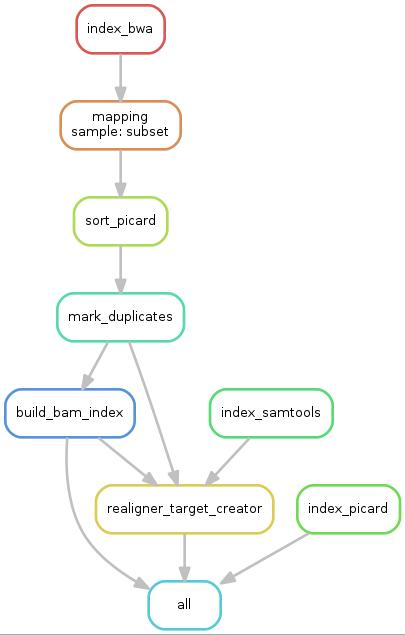
\includegraphics[scale=0.5]{Workflow.jpg}
\caption{Workflow}
\label{fig:workflow}
\end{figure}
L'algoritmo GATK-LOD\ped{n} è stato integrato solo fino al riallineamento di GATK, escludendo quindi i passaggi di riallineamento Indel e di ricalibrazione dei punteggi di qualità.
Allo stesso tempo non sono state considerate le fasi fondamentali di chiamata alle varianti e l'implementazione del classificatore LOD\ped{n} di MuTect, vera novità del metodo GATK-LOD\ped{n}.

Questa forte selezione degli step è stata voluta appositamente per non appesantire lo studio sull'ottimizzazione computazionale e, quindi, è stato scelto di concentrare le analisi solo su quelle operazioni che formano le basi dell'algoritmo genetico.
In tale maniera, è facilitato sia l'indagine sulla scalabilità che il confronto tra i diversi apparecchi adoperati, così da poter trarre rapidamente le prime conclusioni.



\subsubsection{Organizzazione dei prodotti}
Il materiale su cui sono condotte le analisi statistiche sono i particolari tecnici e tempistici di ognuna delle regole completate.
Tali dati sono procurati, come già spiegato nel \textbf{capitolo Snakemake}, dalla direttiva benchmark in ogni passaggio.
Ciò significa che al termine dell'algoritmo sono prodotti tanti singoli file di benchmarking quante regole sono state completate, contando pure il caso in cui esse venissero ripetute ricorsivamente.
Per controllare la quantità di file e agevolare il futuro studio statistico, è stato scritto uno script in Python, denominato \verb!script_benchmark!.


Ogni file benchmark è dotato di un nome avente funzione di etichetta; in particolare, la forma è la seguente.
\begin{lstlisting}
benchmark_{name}_subset_{sample}_n_sim_{n_sim}_cputype_{cpu_type}_thrs_{thrs}_ncpu{n_cpu}.txt
\end{lstlisting}
Gli attributi contenuti nel nome indicano ordinatamente: il nome della regola completata, il tipo di campione analizzato, il numero della simulazione, il tipo di cpu utilizzata e il numero di threads e di cpu adoperati.
Mentre i primi due sono ricavati in automatico, gli altri fanno riferimento al file di configurazione dello Snakefile, come sarà spiegato nel paragrafo seguente.

Il lavoro svolto dallo script consiste quindi nel leggere ognuno dei file benchmark generati, considerare le etichette delle simulazioni e trasferire i dati incolonnati in un'unica tabella.
La tabella risultante non è dotata, quindi, solo delle colonne predefinite da \textit{Snakemake} nell'operazione di benchmarking(presentate nella sezione \textbf{benchmark} della sezione 1.2), bensì è arricchita dai dettagli contenuti nell'etichettatura.
In particolare, i dati sono organizzati nella tabella in ordine crescente rispetto al numero di simulazione.

Il nome prestabilito per la tabella si può ritrovare nel codice sorgente dell'eseguibile ed è necessario accedere ad esso e modificare tale nominativo se si desidera crearne una nuova.
Difatti, all'avvio dello script è controllato se sia presente una tabella con lo stesso nome: in caso affermativo, i nuovi dati sono accodati ai precedenti; al contrario, ne è inizializzata un'altra.

Attraverso questo sistema, il prodotto finale della fase di esecuzione, ed un unico oggetto dell'analisi statistica, è una tabella che racchiude le proprietà relative alle simulazioni ultimate.


Prima di procedere con l'esposizione dello studio effettuato su tali tabelle, è indispensabile perfezionare la descrizione del procedimento, specificando le opzioni di configurazione su cui essa si struttura.


\subsection{Configurazione}
Le ultime componenti del procedimento da delineare sono le modalità che definiscono le condizioni sotto cui deve essere portata avanti la computazione.
Queste componenti sono riportate nei file di configurazione e, in questo progetto, sono stati scritti due file di questo tipo che corrispondono rispettivamente a \textit{Snakemake} e a \textit{Conda}.

Le informazioni necessarie allo Snakefile sono procurate dal file \textit{config.yaml} che comunica a \textit{Snakemake} alcuni dettagli della simulazione e le indicazioni su certe dipendenze.


Gli attributi della simulazione completano semplicemente l'etichettatura dei file di benchmarking e, pur rivestendo uno ruolo marginale, tali etichette permettono allo script di organizzazione dei dati una lettura rapida e quindi un'istanza immediata della tabella.
Come già citato precedentemente, i dettagli trascritti nel file di configurazione sono il tipo di cpu sfruttata, il numero della simulazione, il numero di threads adoperati e il numero di cpu coinvolte.

E' stato scelto di gestire queste informazioni come parametri per non irrigidire il programma, visto che gli apparecchi e i meccanismi usati possono essere innumerevoli.
Nello specifico, per modificare questi dettagli nelle etichette è sufficiente agire da linea di comando, come indicato nel paragrafo 1.2.1.

Sempre nello stesso file di configurazione sono presenti alcune chiavi che rappresentato le dipendenze non implementabili direttamente negli ambienti di \textit{Conda} per \textit{Snakemake}.
Innanzitutto, sono presenti due indicazioni necessarie per il meccanismo di mapping, che sono l'utilizzo di \textit{Illumina} come piattaforma e di \textit{WES-Nextera-Rapid-Capture} come libreria.
A seguire, è indicato l'indirizzo in cui si può trovare il Genome Analysis ToolKit, da applicare nella procedura di riallineamento.

Altre istruzioni sulla configurazione del procedimento sono richieste da \textit{Conda} per la creazione, attivazione e disattivazione degli ambienti di lavoro durante l'esecuzione di \textit{Snakemake}(paragrafo 1.2.1).

Nell'ambito di questa ricerca, è stato scritto solo un documento di configurazione relativo a \textit{Conda}, dato che la maggior parte dei processi necessita di un ambiente con le stesse caratteristiche.
Nello specifico, quest'unico file di riferimento è contenuto nella directory \textit{envs} ed è chiamato \verb!config_conda.yaml!.

I requisiti richiesti per l'ambiente sono soddisfatti istruendo espressamente \textit{Conda} all'utilizzo del canale \textit{bioconda} per procedere con l'installazione di tre software coinvolti nel sequenziamento: \textit{BWA}, \textit{Picard} e \textit{Samtools}.

Ora che l'ossatura del sistema è stata argomentata e sono stati approfonditi pure le procedure configurative, è possibile illustrare il percorso di studio statistico effettuato, accompagnato da una presentazione del genere di simulazioni conseguite.

\section{Studio statistico}
